\section{Introduction}
A community question and answer (Q\&A) website provides a collaborative information seeking platform for users to ask and answer questions.
The accumulated questions and answers over time create a crowdsourced knowledge base which can benefit many people (in addition to the question askers themselves) who have similar questions.
Recent years have witnessed the unprecedented development of Q\&A websites such as Stack Exchange and Quora. 

\begin{comment}
\begin{figure}
	\centering
	\subfigure[Spanish Stack Overflow]{%
		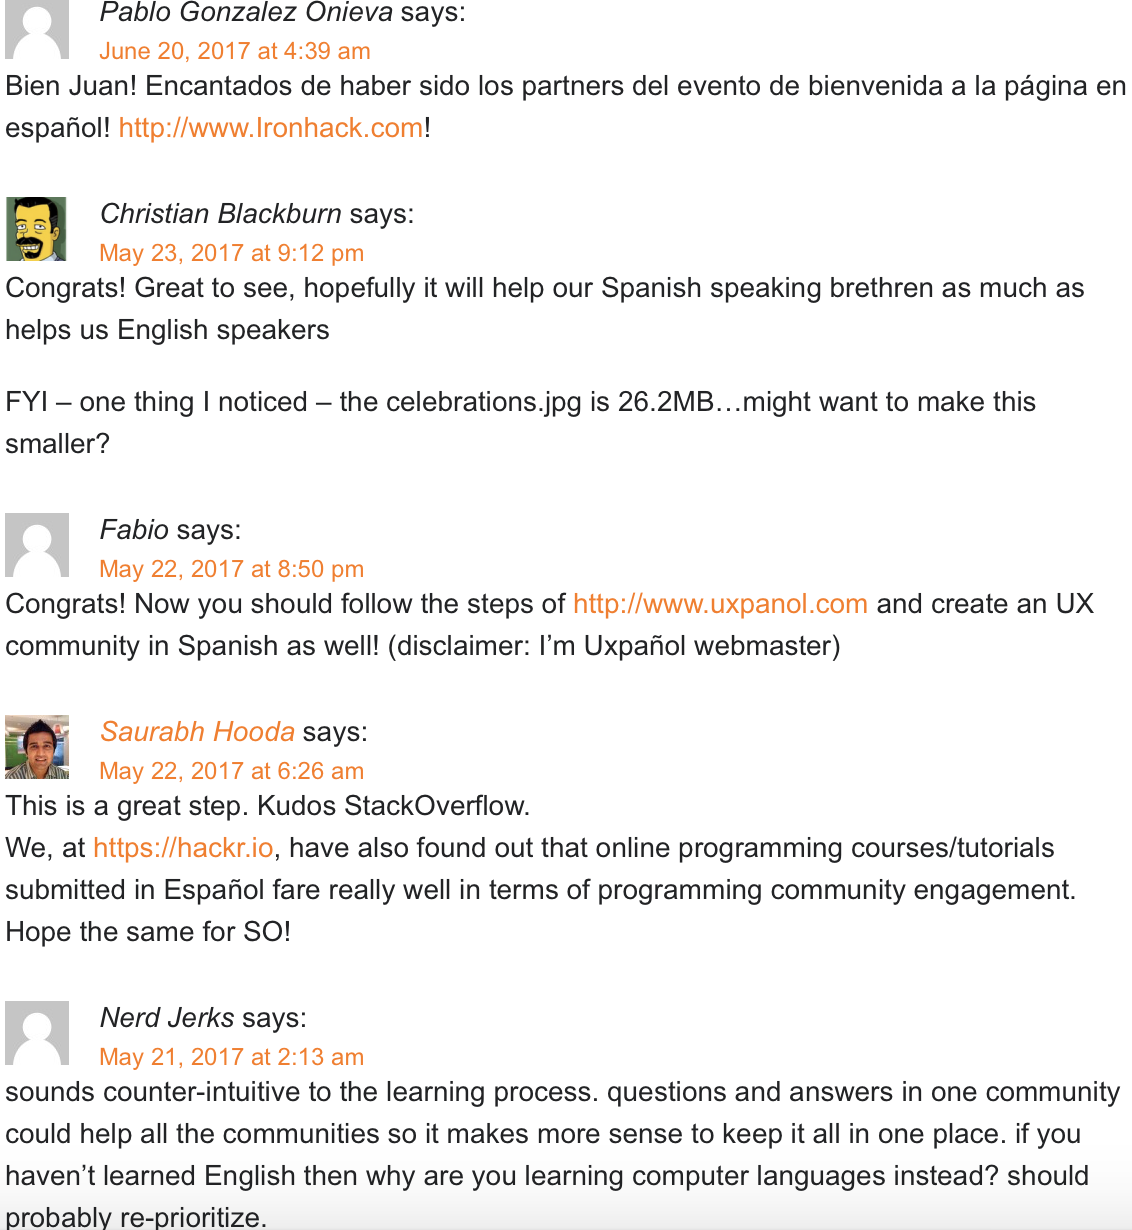
\includegraphics[width=0.42\textwidth]{figures/SOcomment.png}
		\label{fig:SOcomment}
	}
	\hfill
	\subfigure[Spanish Quora \textcolor{red}{suggest not to use Quora. Consider using a post example on Meta Stack Overflow}]{%
		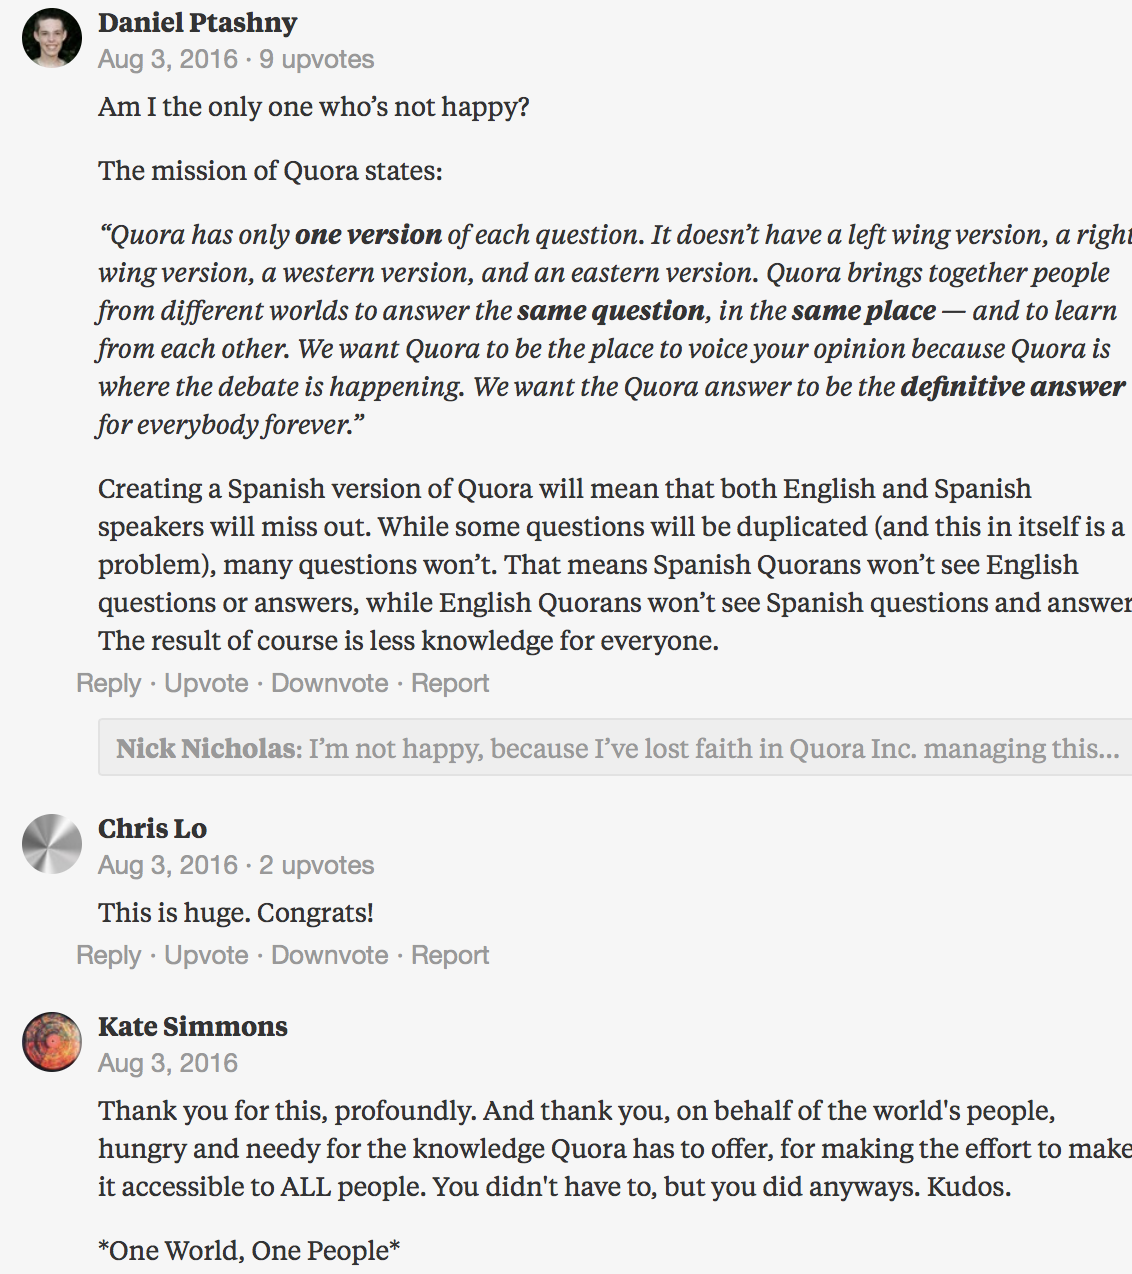
\includegraphics[width=0.42\textwidth]{figures/QuoraComent.png}
		\label{fig:QuoraComment}
	}
	\caption{Example user comments and discussions on the launching of multi-lingual Stack Overflow sites
		\textcolor{red}{
			1) I say not to show Quora example here. Quora is for general domain which may have completely different phenomena from Stack Overflow. It is very likely that our findings on Stack Overflow cannot be extended to Quora. And this will invite questions why not study both Stack Overflow and Quora and contrast them to gain even deeper insights. I say if we really want to discuss Quora, mentioning it only in the Discussion section as future work.
			2) Still use two examples. One from the comments left on the announcement. The other from the separate post discussion. No need to use screenshots. Very hard to read. Instead, use a table or so to quote the comments. 
			3) Organize the comments into three parts: community split, knowledge interests, knowledge fragmentation/duplication. For each part, list one or two supporting comments and one or two against comments. Highlight key phrases in the comments to attract the readers' attention. 
		}
	}
	\label{fig:userComments}
\end{figure}
	
\end{comment}
  
\begin{figure}
	\centering
	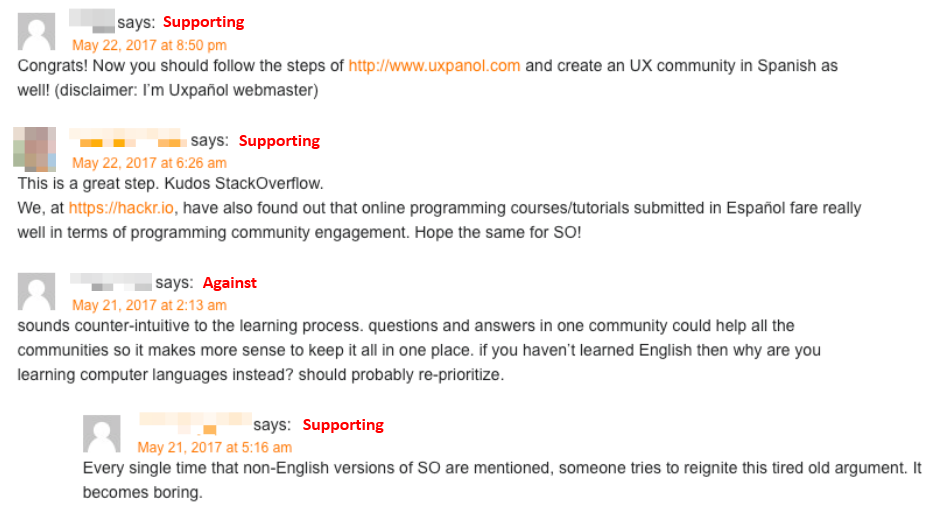
\includegraphics[width = 0.95\textwidth]{figures/SpanishSO.png}
	\caption{Example user comments and discussions on the launching of Spanish Stack Overflow site~\cite{web:SOspanish}}
	\centering
	\label{fig:userComments}
\end{figure}  

Originally, most of the Q\&A sites run in one language (mostly English).
However, %English is only one of \textcolor{red}{xxx} languages in the world.
for those who do not speak English or do not use English as their working language, they cannot directly access such English Q\&A sites due to the language gap.
%However, this non-English population is a big potential market for a successful English Q\&A site to extend its business.
To make the site available for non-English population, many Q\&A sites begin to release their multi-lingual variants to serve users who speak other languages.
Note that a multi-lingual variant of a Q\&A site is neither the translation version of the original English site, nor the original site with language localisation features.
Instead, it is a totally new site for a non-English language but adopts the same policies, practices and supports the same look and feel and user experience as the original English site.
For example, there are Russian, Japanese, Portuguese, Spanish Stack Overflow\footnote{\url{https://stackoverflow.blog}}, and French, Spanish, Japanese, German, Italian Quora\footnote{\url{https://blog.quora.com}}.
Despite these benefits, the decisions of launching some multi-lingual variants of the original English site always cause intense dispute about the pros and cons of multi-lingual variant sites among users.
This is evident from the supporting- or against-comments that users left on the announcement of the new multi-lingual sites~\cite{web:SOjapanese, web:SOportugese1, web:SOportugese2, web:SOrussian, web:SOspanish}.
Users also created some posts on Meta Stack Exchange and Meta Stack Overflow to discuss the points in favour of or against multi-lingual sites~\cite{web:SOdiscussion1, web:SOdiscussion2, web:SOdiscussion3, web:SOdiscussion4, web:SOdiscussion5, web:SOdiscussion6, web:QuoraDiscussion}.

Fig.~\ref{fig:userComments} presents one typical example of such dispute about the multi-lingual Stack Overflow sites.
We conduct a formative study in which we crawl all the user comments on the launch of multi-lingual Stack Overflow sites.
Three major concerns emerge from our analysis: 
\textit{community split}, \textit{knowledge needs and interests in English and other languages}, and \textit{knowledge fragmentation and duplication}.
On the one hand, users who are against the multi-lingual sites are worried about: this would cause the community split across different sites, whether there are enough needs and interests in computer programming knowledge in other languages, and knowledge fragmentation and duplication across different sites would become a serious issue to deal with.
On the other hand, users who support the multi-lingual sites argue that: the multi-lingual sites could involve more non-English-speaking users in the community, there are different knowledge needs and even unique knowledge interests for non-English-speaking users, and knowledge duplication may not be a bad thing as long as good questions and answers in one language could be referenced or translated in another language.
  
People use different examples, reasons, arguments to defend their opinions, but they can rarely provide solid evidences to convince others, and thus the same dispute repeats once another multi-lingual site is launched.
Some users point out the needs for more evidence-based analysis of multi-lingual sites, rather than just conjecturing what would or would not happen.
For example, this user suggests in his post~\cite{web:SOdiscussion1} that ``\textit{We need to see charts of activity by country to gauge how many people this would bleed away from the main site. My guess is, it's a lot more than you'd expect}''.
With the launch of multi-lingual sites and the data accumulated on these sites over time, it becomes feasible for evidence-based analysis and comparison between the multi-lingual sites and the original English site, which will give us insights into the value of multi-lingual sites, their impacts on the original English sites, and the necessary tools to support the multi-lingual sites.

In this paper, we conduct such an evidence-based data analysis and comparison between the Russian Stack Overflow (RSO) and the English Stack Overflow (ESO).
We choose Stack Overflow as the subject site because it is the most successful and popular Q\&A site for computer programming and it provides up-to-date data dump of the entire site information for public use and research.
We choose Russian Stack Overflow because it is the largest multi-lingual Stack Overflow variant with sufficient users and posts for the comparative study.
Inspired by the three major concerns we identify in our formative study of the user comments on the launch of multi-lingual Stack Overflow sites, we focus our analysis on three points.
First, we study the risk of community split from the user perspective by analyzing user registration, user reputation score, and user posting behavior on RSO and ESO.
Second, we study the knowledge needs and interests in English and Russian from the tag perspective by analyzing tag frequency correlation and tag uniqueness between RSO and ESO.
Third, we study the knowledge fragmentation and duplication issue from the cross-site linking perspective by analyzing existing manual cross-site links by users and potential cross-site links that users are not aware of.

Our results show that some special knowledge needs and interests in non-English languages warrant the value of multi-lingual Q\&A sites, and multi-lingual Q\&A sites do not result in community split.
However, knowledge fragmentation and duplication across multi-lingual sites is a valid concern.
Although manual cross-site linking can partially deal with this issue, the extent of knowledge fragmentation and duplication calls for automated cross-site linking and cross-site translation support.

%Therefore, in this work, we carry out data-driven empirical study to check the main pros and cons quantitatively.
    
%We first summarise users' opinions from their comments under the announcement of multi-lingual new sites in Stack Overflow blogs.
%The pros and cons are concluded as the motivation of this work.
%We especially take the Stack Overflow and Russian Stack Overflow as the case study to investigate the mutual influence between two sites.
%We then analyse their relationships from different aspects such as 
%.....

The main contributions of this paper are listed below:	
\begin{itemize}
	\item This work is the first quantitative study of the phenomena and effects of multi-lingual Q\&A sites. 
	It provides evidences to validate the existence value of multi-lingual Q\&A sites, the risk of community split, and the issue of knowledge fragmentation and duplication. 
	%variants and validates the concerns of the community split and duplicate content in the new site, but the effects are rather small. 
	\item Our study identifies a new problem for the development of multi-lingual Q\&A sites, i.e., manual cross-site linking is not sufficient for bridging the knowledge across multi-lingual sites. We provide a cross-site retrieval method which has potential to tackle this problem. 
	%\textcolor{red}{CCY: I think we need to tune down for our cross-site retrieval method.}
	\item Inspired by our findings, we envision cross-site retrieval and cross-site translation techniques to better support multi-lingual Q\&A sites, and identify key challenges in developing such techniques.
	%based on our discovery to assist new sites. The tool is needed for helping locate reference of old questions in the main site, and translate accepted answer to target language.
\end{itemize}

\begin{comment}
	
	Stack Overflow is a platform with millions of users and huge amount of content. Table 1 presents the statistics of users, posts and comment Stack Overflow main site and other lingual sites. As shown, the number of users as well as the amount of posts and comments in the English main site are much higher than the other multilingual sites. Also, there are only 50\% to 60\% of the lingual variant users who also use the Stack Overflow main site at the same time. This indicates that a considerable sum of users only use the lingual variant site which means they may ask or answer some questions already existing on the main site.
	
   	To get more potential users over the world and extend the current business model, setting up the new multilingual sites based on Tehran current English main site has been a very popular strategy for the English Q\&A websites. So does Stack Overflow. Since Ethe coding language are developed and based on the English Stack Overflow, a codeing Q\&A website, were originally developed in English and it has become the msot popular coding Q\&A website in the world. It also starts to run the multilingual sites aiming to different programer communities in other languages. Because the native language is much more attractive for the native speakers, and the long term goal of Stack Exchange Network is to be a great and planetary resource for worldwide citizens no matter what language they speak [8].
\end{comment}
   	
   	
   	%To get more potential users over the world and extend the current business model, setting up the new multilingual sites based on the current English main site has been a very popular strategy for the English Q\&A  websites. So does Stack Overflow. Since the coding language are developed and based on the English, Stack  Overflow, a coding Q\&A website, were originally developed in English and it has become the most popular coding  Q\&A website in the world. It also starts to run the multilingual sites aiming to different programmer communities in other languages. Because the native language is much more attractive for the native speakers, and the long term goal of Stack Exchange Network is to be a great and planetary resource for worldwide citizens no matter what language they speak [8].
   
\begin{comment}	
   	Therefore, it is meaningful if a clear answer can be found when websites and communities keep developing their multilingual variants, and more contributions is supposed to be made to bridge the lingual gap for all users who are interested in some content on the website writing in other language. It is highly believed that humans are accustomed to a more familiar environment [24], especially lingual environment. Although some people learn a second language, when the question is related to a domain-specific topic with a lot of professional words it is also very hard for them to search, understand or express their thoughts clearly. 
\par
	The active level of a community is determined by many factors, and the most important ones are users and content. Comparing the statistics in Table 1, it is clear that the number of user in Stack Overflow main site is around 90 times that of Russian Stack Overflow, and the content in the main site is also much more than the other multilingual sites which means the gap of their resources may be enormous. To clearly identity and quantitatively analysis this difference,  an empirical study on the users and content between the Stack Overflow main site and Russian Stack Overflow has been conducted. The main research object is locked on the Russian Stack Overflow besides the main site, since it has the top number of users and top amount of posts as well as comments than other multilingual variants. 
	\par
	
		There are several interesting cases on the sites of Stack Overflow, which are presented in Figure 1. The sub-figure a) shows a very common phenomenon that users from the other lingual sub-site of Stack Overflow like the Russian variant often cannot find satisfying and high-quality answers on other lingual Stack Overflow sites, which need to be defined as {\bf sub-sites}, for some reasons, while the main site can always assists them with the solutions. The sub-figure b) is a answer posted on Russian Stack Overflow, which means, in English, there are some previous solutions on the Stack Overflow English main site for this specific Russian question. 
\par
	Imagine that a Russian speaker who cannot speak English fail to find a good answer to his or her question. Meanwhile, the reply to his post is quite slow because the number of users on Russian Stack Overflow is small. For this problem, our cross-lingual question retrieval model can efficiently deal with the lingual gap problem and recommend useful resources across different languages. A key benefit of this approach is the non-English speakers can efficiently utilize the huge knowledge base from the dominant English community.
\end{comment}   	
	

